

\actTitle{Worksheet 4.1}


\noindent \textbf{Instructions:}  Work together in groups of  3 or 4 to complete the following problems.\\

Student goals:
\begin{itemize}
\item Determine an angle's measurement in radians given the arc length
  and radius of a sector.
\item Place an angle in standard position given a verbal description.
\item Determine the terminal or the initial side of a sector.
\item Recognize whether an angle is positive, negative or zero.
\item Recognize when two angles have coterminal sides.
\item Given any two values of a sector's radius, angle, or arc length
  determine the value of the remaining quantity.
\item Determine the area of a sector given the radius and angle.
\item Given any two values of a sector's radius, angle, or arc length
  determine the value of the area of the sector.
\item Recognize when a given angle represents more than one complete
  rotation around a circle.
\end{itemize}


For each of the following questions first make a rough sketch of the
relevant figure.
\begin{enumerate}

\item Find a positive angle less than $360^\circ$ that is coterminal with each of the given angles.
\begin{enumerate}
\item  $\theta=400^\circ$\vfill
\item $\alpha=-160^\circ$\vfill
\vfill
\end{enumerate}


\item Find a positive angle less than $2\pi$ that is coterminal with each of the given angles.
\begin{enumerate}
\item  $\displaystyle \beta=-\frac{\pi}{15}$\vfill
\item $\displaystyle \phi=\frac{34\pi}{9}$\vfill
\vfill
\end{enumerate}

\clearpage

\item Find the radian measure of the central angle $\theta$ of a circle of radius $r=8$ meters that intercepts an arc of length $s=14$ meters.
\vfill


\item The minute hand of a clock is 3 inches long.  How far does the tip of the minute hand move in 45 minutes?\vfill

  \clearpage
  
\item The minute hand of a clock moves from 12:10 to 12:30.
\begin{enumerate}
\item How many \textbf{degrees} does it move during this time?\vfill
\item How many \textbf{radians} does it move during this time?\vfill
\item If the minute hand is 10 inches in length, determine the exact distance the tip of the minute hand travels during this time.\vfill
\end{enumerate}

\item Find the exact area of the following sectors given the radius of
  the circle $r$ and the subtended angle $\theta$.  Then round the
  result to the nearest tenth of a unit.

\begin{enumerate}
\item $r=6$ m; $\theta=\frac{5\pi}{3}$\vfill
\item $r=3$ cm; $\theta=120^\circ $\vfill

\end{enumerate}


\clearpage

\item You are one member of a group of 8 friends who are going out for pizza.  A small pizza has a 6" radius, while a large pizza has 9"  radius.  Answer the following questions.
\begin{enumerate}
	\item How much pizza will each of you eat if you order two small pizzas?  Will you get more of less pizza if you order one large pizza? (Assume everyone eats the same amount and all the pizza is eaten.)
	\vfill
	\item How many inches of crust will each person eat if you order two smalls?  If you order one large will you get more crust?
	\vfill
	\item Suppose you and your friends want to order one pizza and that you each want to eat 50 square inches worth of pizza.  What should the radius of the pizza be?
	\vfill
\end{enumerate}

\clearpage

\item The radius of the circle shown in the diagram below is three, and
  the area of the sector defined by the shaded region is 10.5.
  Determine the radian measure of the angle $\psi$.

  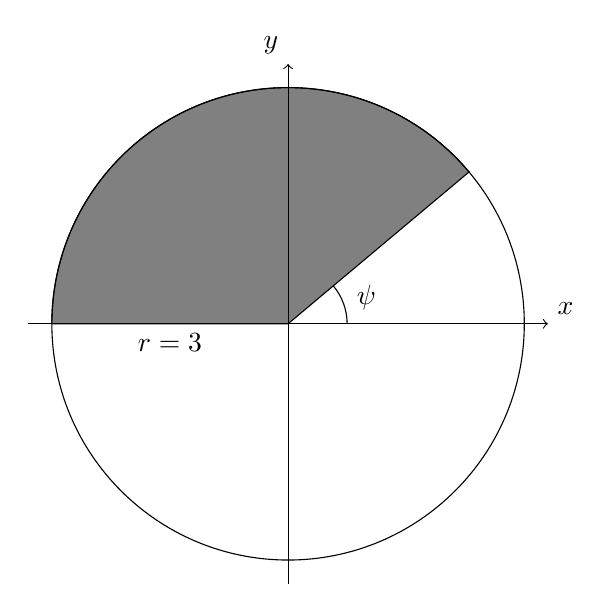
\begin{tikzpicture}[y=1.5cm, x=1.5cm,font=\sffamily]
    \draw[thin,black,fill=gray] (0,0) -- (40:2) arc (40:180:2) -- (0,0);
    %\draw[very thick,black] (40:2) arc (40:180:2);
    \draw[black] (0,0) circle (2);
    \draw[black] (0:.5) arc (0:40:.5) node[pos=0.1,anchor=south west] {$\psi$};
    % \node[xshift=0] at (145:0.7) {$\delta$};
    % \draw[thin,black] (110:0.3) arc (110:180:0.3);
    \draw[thin,black,->] (-2.2,0.0) -- (2.2,0.0) node[anchor=south west] {$x$};
    \draw[thin,black,->] (0.0,-2.2) -- (0.0,2.2) node[anchor=south east] {$y$};
    \node[black,anchor=north] at (-1,0) {$r=3$};
    % \node[black,anchor=south west] at (55:2) {$s$};
  \end{tikzpicture}

  \vfill

\item A wheel with a diameter of 0.7m rolls a distance of 400m. What angle did it turn?

  \vfill
    

\end{enumerate}


\hwTitle{Section 4.1}

\begin{enumerate}
  \item Suppose that the three circles drawn below have radii of length 1, 2, and 3.  For each pair of points given below, find the shortest path connecting the points.
%\vspace{-1in}
\begin{center}
  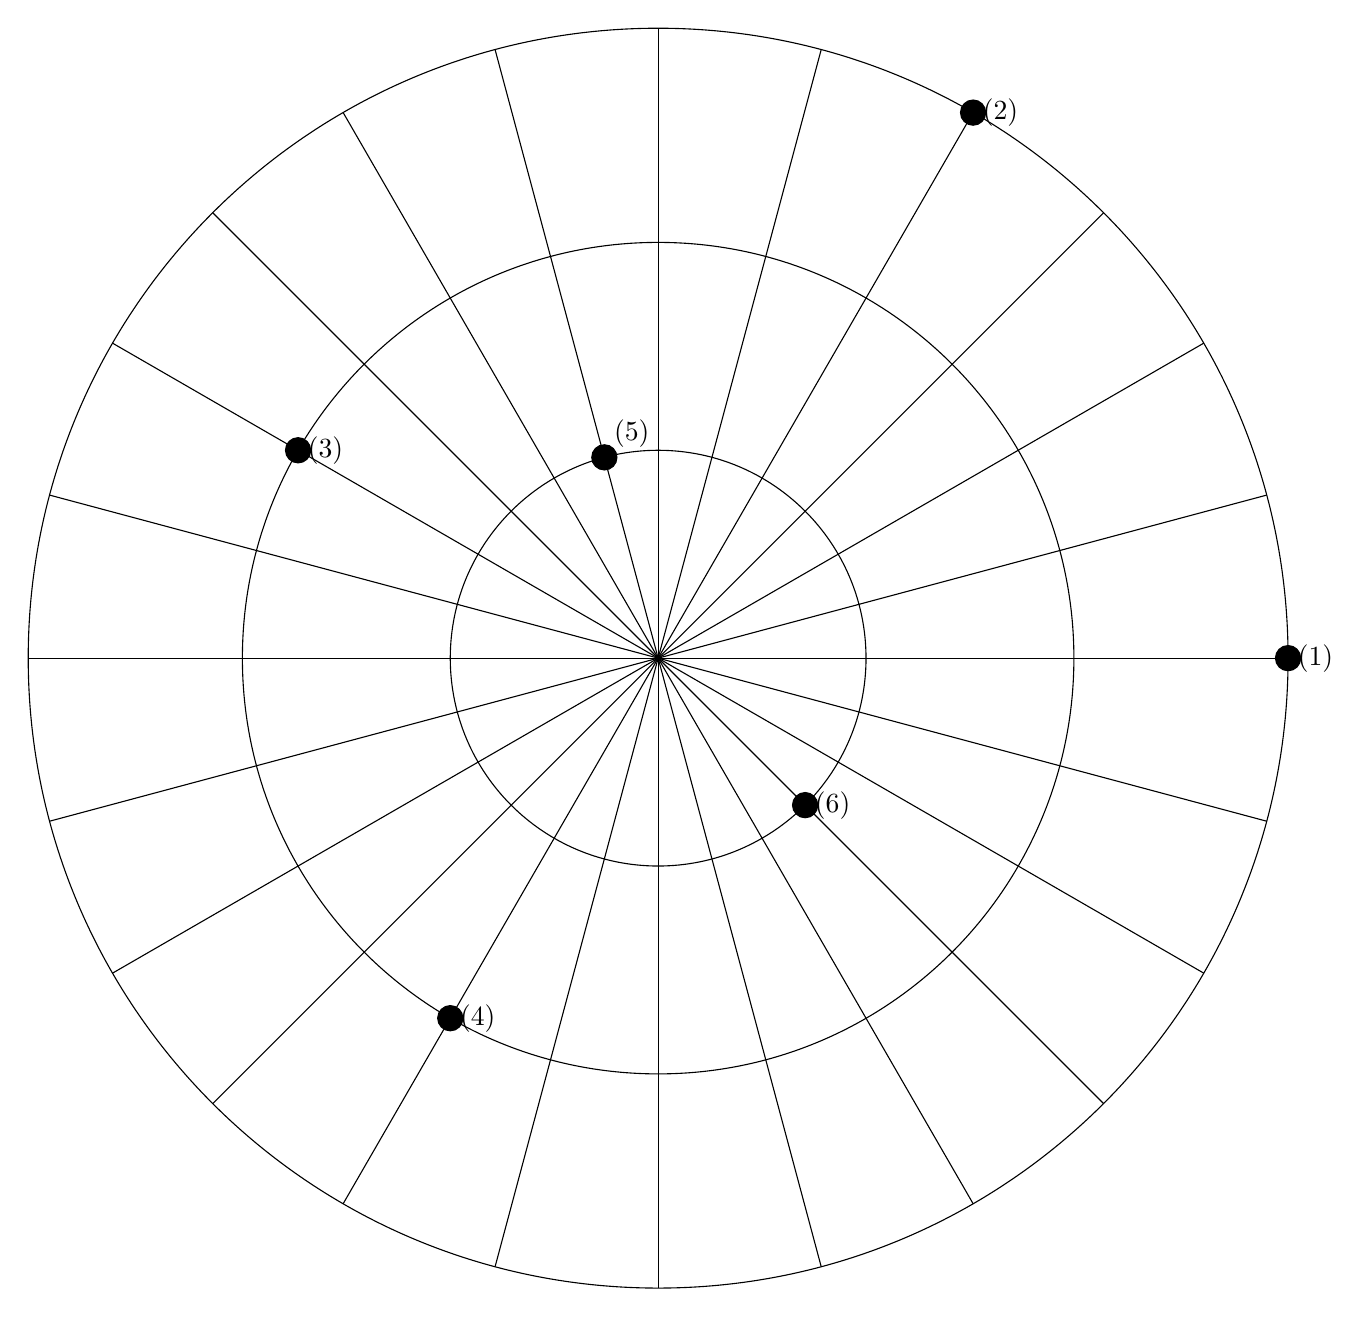
\begin{tikzpicture}[scale=8]
    \foreach \t in {0,15,30,...,345} {
      \draw[-] (0,0) -- (\t:1);
    }   
    \draw (0,0) circle(1);
    \draw (0,0) circle(0.66);
    \draw (0,0) circle(0.33);
    \filldraw[black] (1,0) circle (0.02) node[anchor=west] {(1)};
    \filldraw[black] (60:1) circle (0.02) node[anchor=west] {(2)};
    \filldraw[black] (150:0.66) circle (0.02) node[anchor=west] {(3)};
    \filldraw[black] (240:0.66) circle (0.02) node[anchor=west] {(4)};
    \filldraw[black] (105:0.33) circle (0.02) node[anchor=south west] {(5)};
    \filldraw[black] (315:0.33) circle (0.02) node[anchor=west] {(6)};
  \end{tikzpicture}
\end{center}



%\vspace{-1in}
\begin{enumerate}
\begin{multicols}{3}
	\item From (1) to (2).
	\item From (3) to (4).
	\item From (5) to (6).
	\item From (3) to (5).
	\item From (2) to (4), \\
	avoiding the center
\end{multicols}
\end{enumerate}




\item Find the exact area of the following sectors given the radius of
  the circle $r$ and the subtended angle $\theta$.  Then round the
  result to the nearest tenth of a unit.
  \begin{enumerate}
  \item $r=1.2$ ft; $\theta=\frac{\pi}{6}$\vfill
  \item $r=2.1$ ft; $\theta=\frac{11\pi}{6}$\vfill
  \end{enumerate}
\end{enumerate}
